\documentclass[11pt]{article}

\usepackage[margin=0.85in]{geometry}
\usepackage{graphicx}
\usepackage{booktabs}
\usepackage{amsmath,amssymb}
\usepackage{hyperref}
\usepackage{xcolor}
\usepackage{enumitem}
\usepackage{float}
\usepackage{subcaption}
\usepackage{microtype}

\hypersetup{
  colorlinks=true,
  linkcolor=blue!50!black,
  urlcolor=blue!50!black
}

\title{\textbf{Technical Speaking Script for Evaluation}\\
\large Notebook-by-Notebook Walkthrough: Evidence-Efficient Diagnostic Workup on DDXPlus}
\author{Baseline Model Research Project}
\date{May 9, 2026}

\begin{document}
\maketitle

\section*{How to Use This Script}

This is written as a speaking guide. The main flow is chronological: baseline first, then LLM-only sequential workup, then MLP-guided stopping, then graph/Bayes methods, then branching.

The short thesis is:

\begin{quote}
We built a DDXPlus diagnostic workup system that starts from incomplete evidence, asks a small number of controlled follow-up questions, and uses a partial-evidence MLP to decide when enough evidence has been collected.
\end{quote}

\section*{1. Problem Setup}

I would start by saying:

This project is about diagnosis under incomplete evidence. DDXPlus gives each case age, sex, an initial evidence field, hidden evidence fields, and one of 49 pathologies.

So our task is not just:

\begin{quote}
Given the full patient record, predict the disease.
\end{quote}

Our task is:

\begin{quote}
Given only initial evidence, decide which evidence to ask for next, update the patient state, and stop when diagnosis is reliable.
\end{quote}

This is why the project is closer to active feature acquisition than plain classification.

\[
U(\pi)=\text{Accuracy}-\lambda \mathbb{E}[N_{\text{requests}}]
\]

That formula captures the basic tradeoff: be correct, but do not ask unnecessary evidence questions.

\section*{2. Notebook 01: One-Shot BASD-Style MLP Baseline}

We first built a serious neural baseline, not a toy baseline.

The baseline follows the BASD style from DDXPlus. In simple terms, BASD means we encode the structured patient state into evidence slots. Each evidence slot can be present, absent, or unknown:

\[
x_j =
\begin{cases}
1, & \text{present},\\
-1, & \text{absent},\\
0, & \text{unknown}.
\end{cases}
\]

The model is an MLP with hidden layers $[2048, 2048, 2048]$ and a softmax over 49 diseases:

\[
\hat{p}(D=k\mid x)=\frac{\exp(z_k)}{\sum_{j=1}^{49}\exp(z_j)}.
\]

The loss is standard cross entropy:

\[
\mathcal{L}=-\log \hat{p}(D=y\mid x).
\]

Result: the initial-evidence MLP reaches about 37.8 percent accuracy on the full test split.

What this proves: initial evidence alone is not enough.

\section*{3. Notebook 07: Full-Evidence Ceiling}

Then we trained the same kind of structured MLP with all evidence visible.

That model reaches about 99.6 percent accuracy.

This is not our live task. It is a ceiling. It tells us DDXPlus has enough diagnostic signal when the right evidence is visible.

\begin{table}[H]
\centering
\begin{tabular}{lccc}
\toprule
System & Accuracy & Top-5 & Evidence \\
\midrule
Initial-evidence MLP & 0.378 & 0.730 & initial only \\
Partial-evidence MLP & 0.515 & 0.827 & sampled partial states \\
Full-evidence MLP & 0.996 & 1.000 & all fields \\
\bottomrule
\end{tabular}
\end{table}

So the scientific gap is clear:

\begin{quote}
How do we choose a small useful subset of evidence?
\end{quote}

\section*{4. Notebooks 02--06: Sequential LLM Workup and Evidence Ledger}

After the one-shot baseline, we moved to a sequential environment.

The key object is the evidence ledger. It is the source of truth for a case.

At the start, the ledger contains:

\begin{itemize}[leftmargin=*]
    \item age,
    \item sex,
    \item initial evidence,
    \item hidden evidence by root id,
    \item revealed evidence roots,
    \item request history,
    \item diagnosis history.
\end{itemize}

When the LLM asks for a field, the ledger checks legality. It prevents duplicate questions and applies parent-child gating. Then it reveals the exact DDXPlus value.

The state update is:

\[
O_{t+1}=O_t \cup \{(a_t,x_{a_t})\}.
\]

Here $O_t$ is visible evidence, $a_t$ is the requested evidence root, and $x_{a_t}$ is the revealed value.

This matters because the LLM never sees the hidden full case. It only sees what the ledger has revealed. That makes the workup controlled and auditable.

\section*{5. Notebook 08: LLM-Only Cost-Sensitive Sequential Baseline}

Notebook 08 tested the LLM as a single evidence-acquisition agent.

The LLM sees the ledger and asks for more evidence or stops. We added a cost-sensitive parameter $\lambda$ so the system is not just controlled by an arbitrary max request budget.

The useful result was that $\lambda=0.10$ reached 0.917 accuracy on 24 cases, but it used about 13 requests per case.

\begin{figure}[H]
\centering
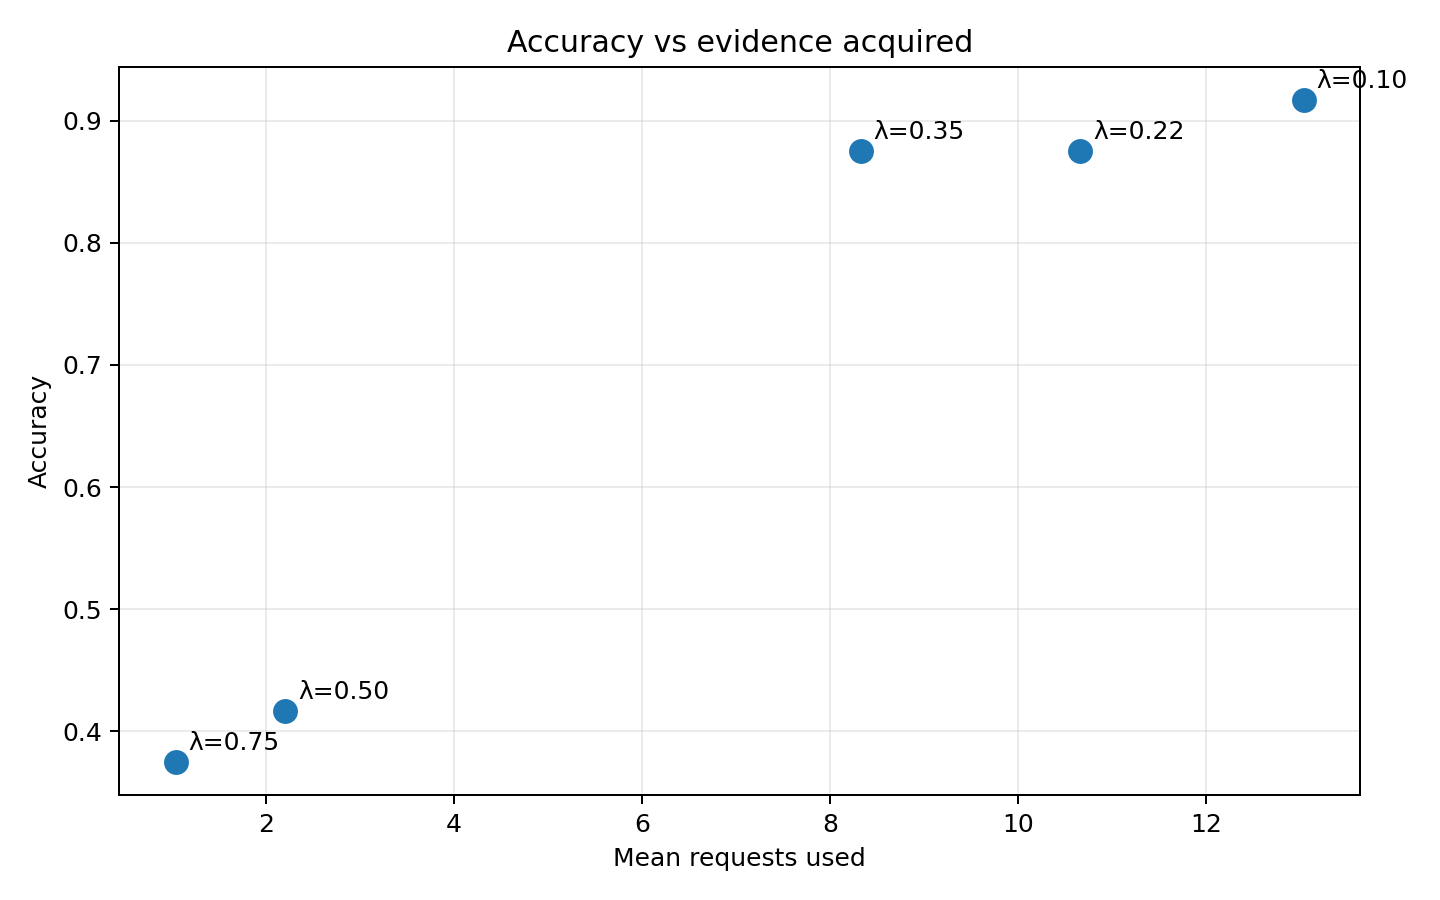
\includegraphics[width=0.78\linewidth]{artifacts/sequential_single_agent_cost_sensitive/single_agent_cost_sensitive_live_test_1perclass_cap24_5lambdas_lambda_cost_24case_wide_sweep_v1/figures/accuracy_vs_mean_requests.png}
\caption{Notebook 08: LLM-only cost-sensitive accuracy versus request count.}
\end{figure}

The lesson was:

\begin{quote}
Sequential evidence acquisition works, but LLM-only stopping is expensive and unstable.
\end{quote}

\section*{6. Notebooks 09--10: Matched-Evidence and Partial-Evidence MLP}

Next we asked a stricter question:

\begin{quote}
Is the LLM good because it reasons better, or because it acquired useful evidence?
\end{quote}

To test that, we trained a partial-evidence MLP. It sees the same style of evidence states that sequential policies create.

The partial-evidence MLP gives:

\[
p_{\text{MLP}}(D\mid O_t)
\]

From that distribution, we compute confidence, margin, and entropy:

\[
c_t=\max_d p_{\text{MLP}}(d\mid O_t)
\]

\[
m_t=p_{\text{MLP}}(d_1\mid O_t)-p_{\text{MLP}}(d_2\mid O_t)
\]

\[
H_t=-\sum_d p_{\text{MLP}}(d\mid O_t)\log p_{\text{MLP}}(d\mid O_t).
\]

Matched-evidence evaluation showed that the acquired evidence itself is valuable. This is why the MLP became part of the live system.

\section*{7. Notebooks 11--13: Final Promoted Hybrid Backbone}

The main promoted method is Notebook 13.

The architecture is:

\[
\text{ledger}
\rightarrow
\text{LLM asks evidence}
\rightarrow
\text{ledger reveals}
\rightarrow
\text{MLP evaluates partial state}
\rightarrow
\text{stop or continue}.
\]

The LLM chooses evidence. The partial-evidence MLP decides whether enough evidence has been gathered.

The selected stop rule is:

\[
c_t \ge 0.70,\quad m_t \ge 0.20,\quad H_t \le 0.10,\quad N_{\text{requests}}\ge 1.
\]

Notebook 12 showed why this mattered. On replay, the selected MLP-guided stop rule reached 0.917 accuracy at about 6.9 requests, while the best pure LLM stop at similar budget reached 0.833.

\begin{figure}[H]
\centering
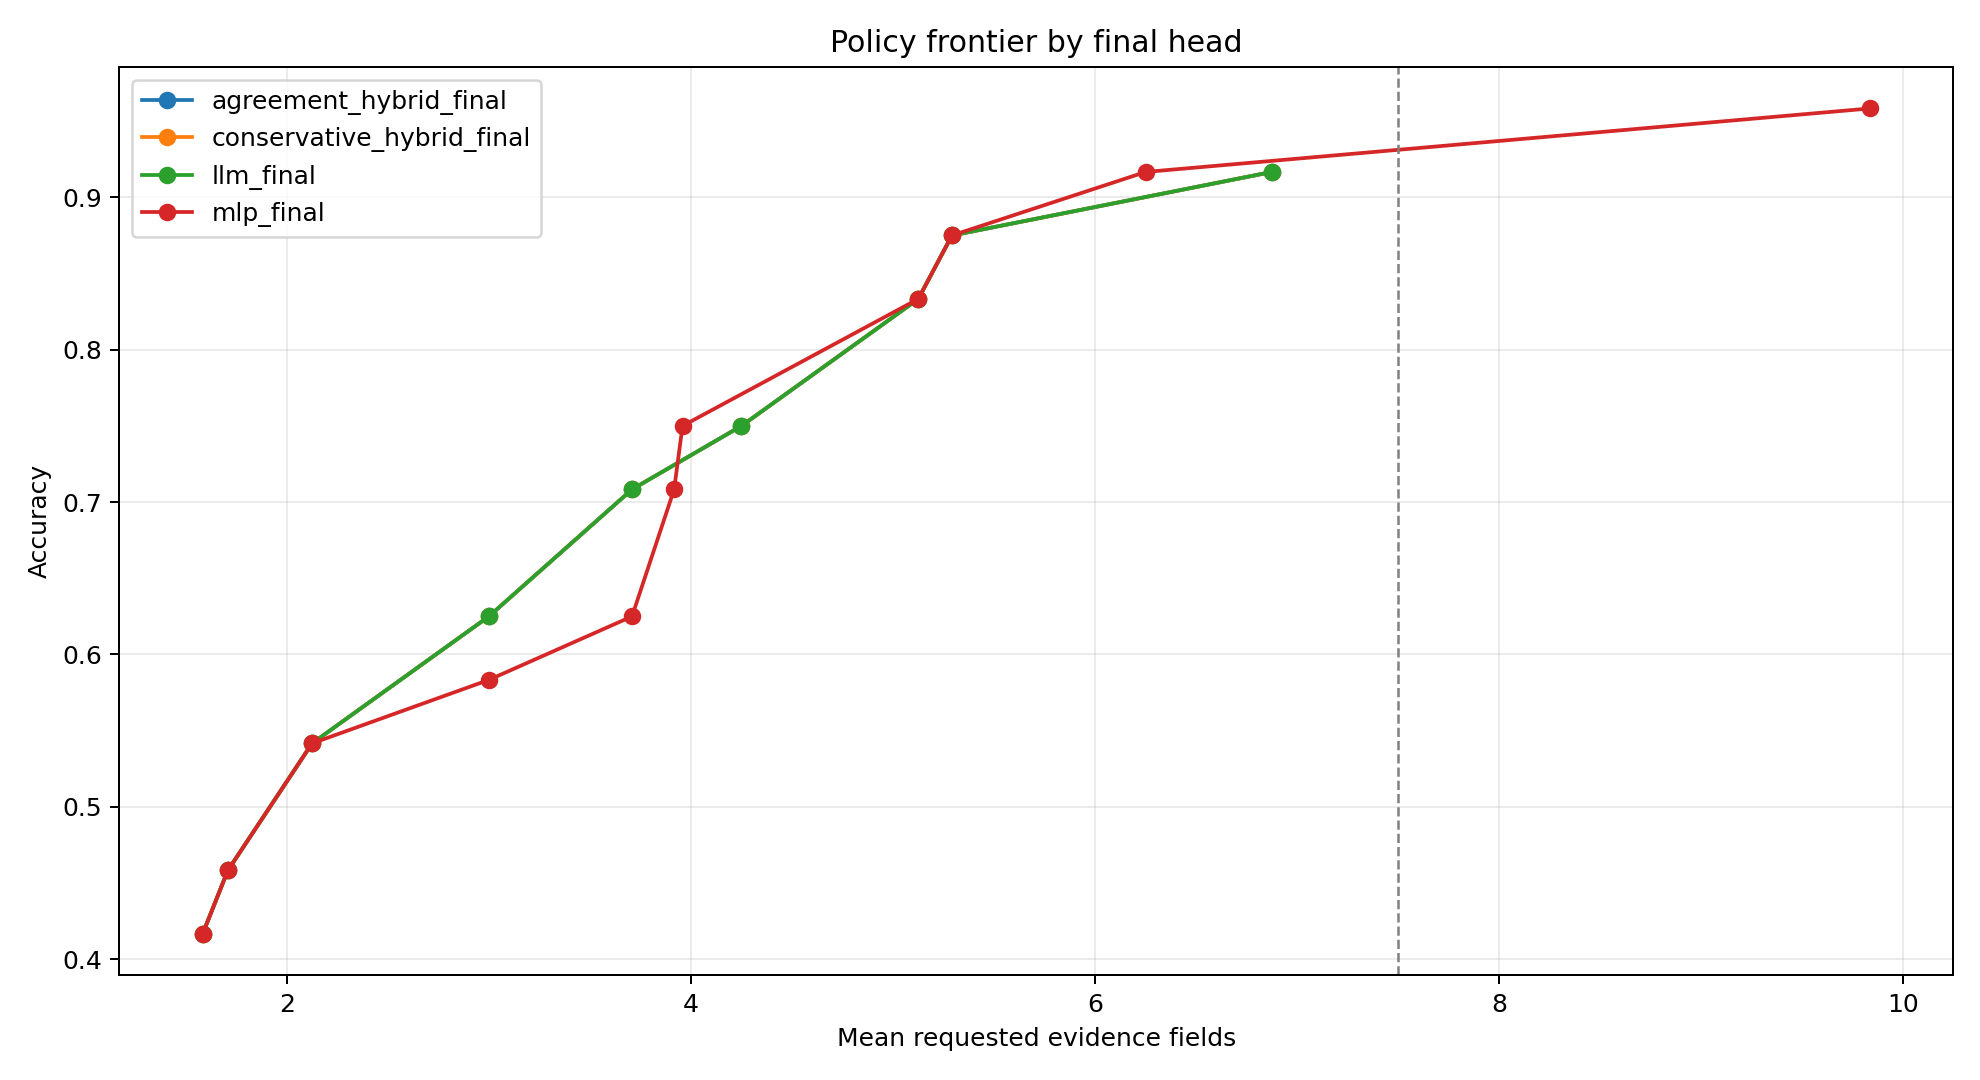
\includegraphics[width=0.78\linewidth]{artifacts/stopping_policy_ablation/stopping_policy_ablation_24case_v1/figures/policy_frontier_accuracy.png}
\caption{Notebook 12: MLP-guided stopping improves the accuracy/request frontier.}
\end{figure}

Notebook 13 confirmed the selected stop rule live:

\begin{itemize}[leftmargin=*]
    \item 43/49 correct,
    \item 0.878 accuracy,
    \item 0.939 top-5,
    \item 6.59 mean requests.
\end{itemize}

\begin{figure}[H]
\centering
\begin{subfigure}{0.48\linewidth}
\centering
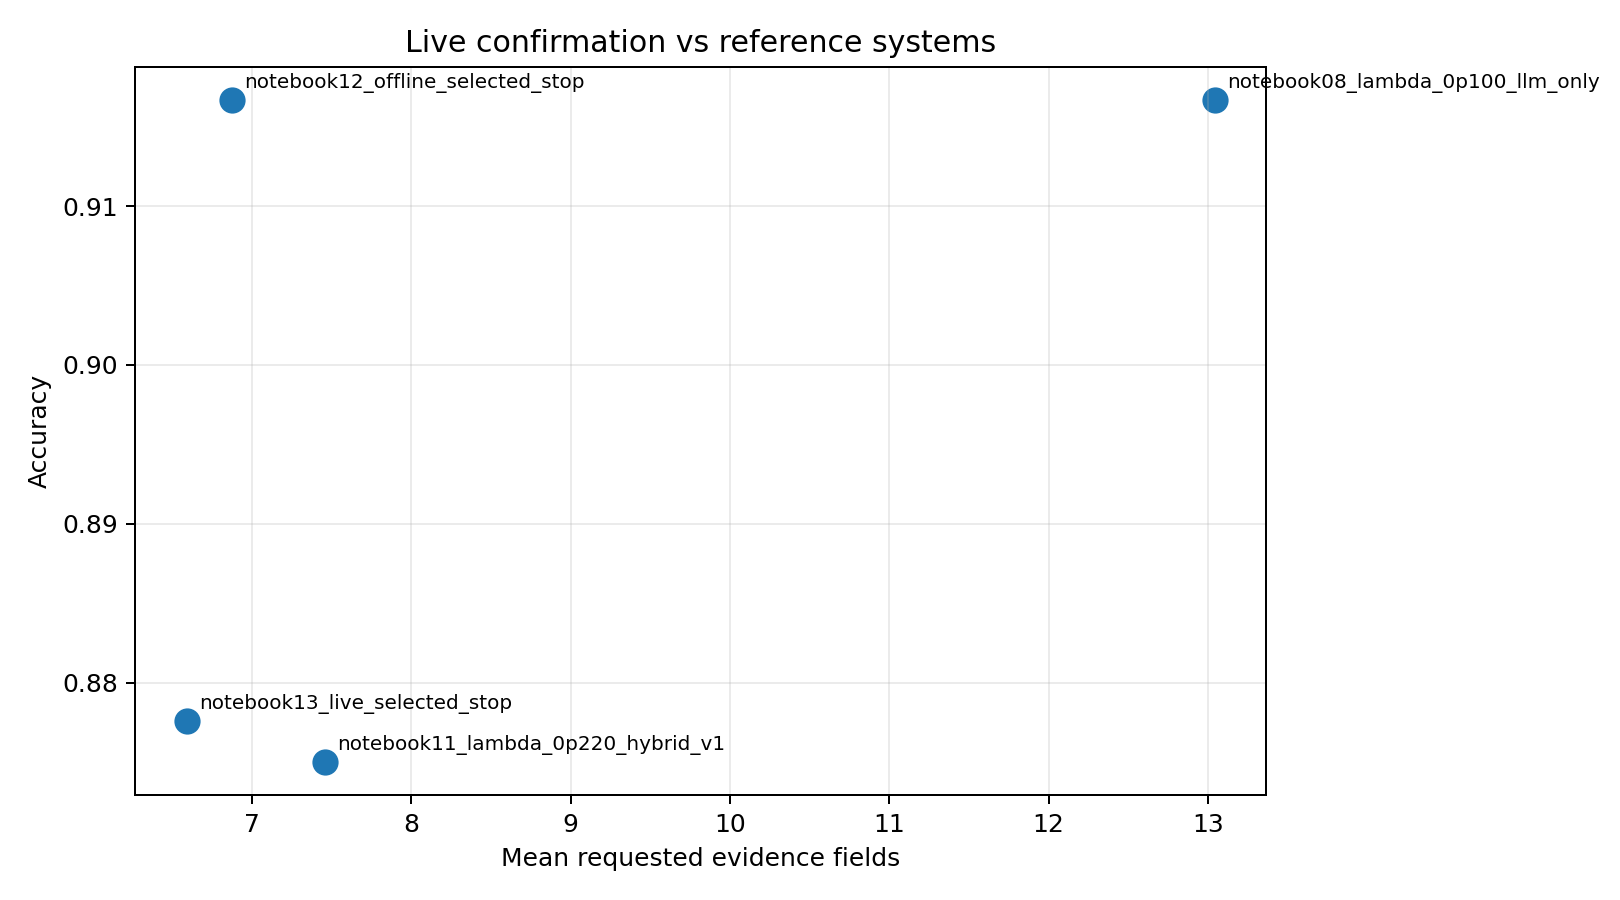
\includegraphics[width=\linewidth]{artifacts/sequential_hybrid_mlp_feedback/selected_stop_live_confirmation_49case_v1/figures/accuracy_vs_reference_requests.png}
\caption{Accuracy vs requests.}
\end{subfigure}
\hfill
\begin{subfigure}{0.48\linewidth}
\centering
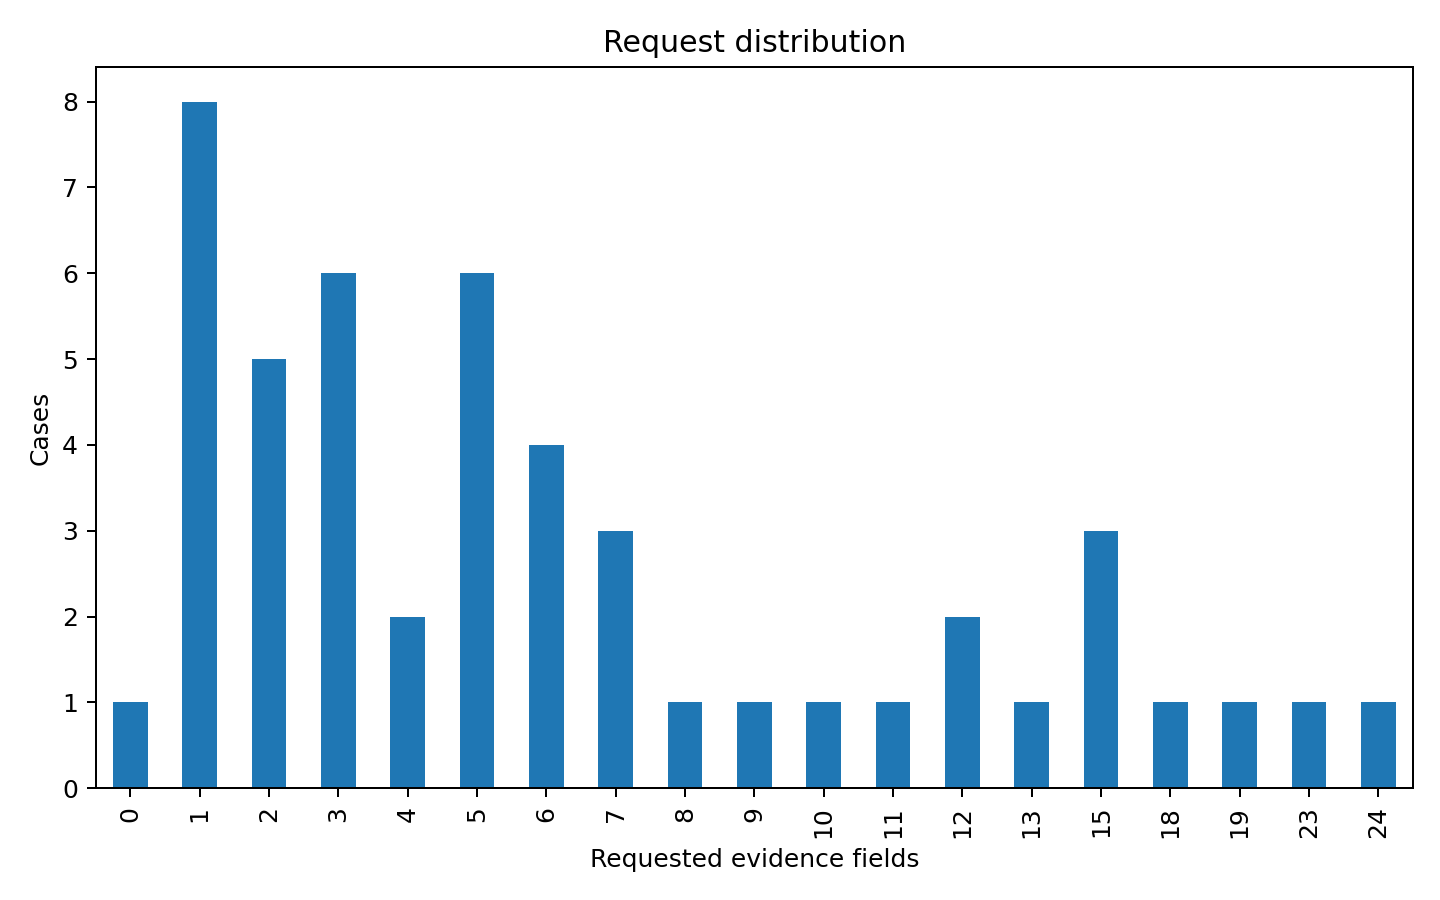
\includegraphics[width=\linewidth]{artifacts/sequential_hybrid_mlp_feedback/selected_stop_live_confirmation_49case_v1/figures/request_distribution.png}
\caption{Request distribution.}
\end{subfigure}
\caption{Notebook 13: final selected-stop live confirmation.}
\end{figure}

This is the backbone I would defend first.

\section*{8. Notebooks 14--15: What We Tried Next}

Notebook 14 asked whether the MLP should also choose questions.

That did not promote. It improved some ranking quality, but top-1 accuracy dropped and request count increased.

The takeaway:

\begin{quote}
The MLP is useful as a belief and stopping monitor, but not automatically better as the question controller.
\end{quote}

Notebook 15 studied stop thresholds and hard-case trajectories. It showed that more evidence is not always better. Some cases drift from correct to wrong after later evidence, especially when the new evidence is generic or points toward a nearby confounder.

\section*{9. Notebooks 16--18: Graph-Ledger Question Selection}

Then we built train-derived graph statistics.

The idea was to connect evidence outcomes to diseases using support and contradiction.

For a disease $d$, the graph score is:

\[
\text{graph\_score}(d)=
\sum_{e\in O_T}\operatorname{clip}(\log \operatorname{odds}(e\rightarrow d),-3,3).
\]

Notebook 16 showed the graph had signal: wrong trajectories had worse graph ranks and weaker graph support.

Notebook 17 tried hard graph top-10 question shortlisting. It underperformed.

Notebook 18 tried graph-advisory shortlisting. It was safer than hard graph replacement but still did not beat Notebook 13.

The lesson:

\begin{quote}
Graph signals are useful, but hard graph control can over-constrain the action space.
\end{quote}

\section*{10. Notebook 19: Bayesian VOI Ledger}

Notebook 19 tried a more mathematical controller: Bayesian value of information.

The posterior is:

\[
P(D\mid E)\propto P(D)\prod_{e\in E}P(e\mid D).
\]

The value of asking a new evidence root is:

\[
\operatorname{VOI}(a)=H(D\mid E)-\mathbb{E}_{x}[H(D\mid E,a=x)].
\]

This is a principled idea: ask the question expected to reduce diagnostic uncertainty.

But empirically it failed. The best fused result reached 33/49 and used 22.37 requests. It asked many globally informative but generic fields, and it created trajectories that the partial-evidence MLP was not trained for.

The lesson:

\begin{quote}
Posterior control is mathematically clean, but trajectory quality and calibration matter.
\end{quote}

\section*{11. Notebooks 20--24: Graph Context, Graph Critic, and Graph/Bayes Rescue}

Notebook 20 added graph context to the LLM prompt instead of replacing the controller. It improved ranking quality but not top-1.

Notebook 21 analyzed graph context as a critic and showed that graph contradiction flags some wrong top-1 answers.

Notebook 22 used graph scoring as a final critic over Notebook 13 evidence. It improved the saved 49-case trace from 43/49 to 44/49 without new requests.

Notebook 23 made this stronger offline. It used graph support, Bayesian posterior, MLP signals, prior recovery, and up to three rescue questions. It improved the saved Notebook 13 trace from 43/49 to 47/49 with zero regressions.

Notebook 24 tested that rescue live. The fresh base itself reached 45/49, but the live rescue also ended at 45/49. So the rescue was not promoted.

\begin{figure}[H]
\centering
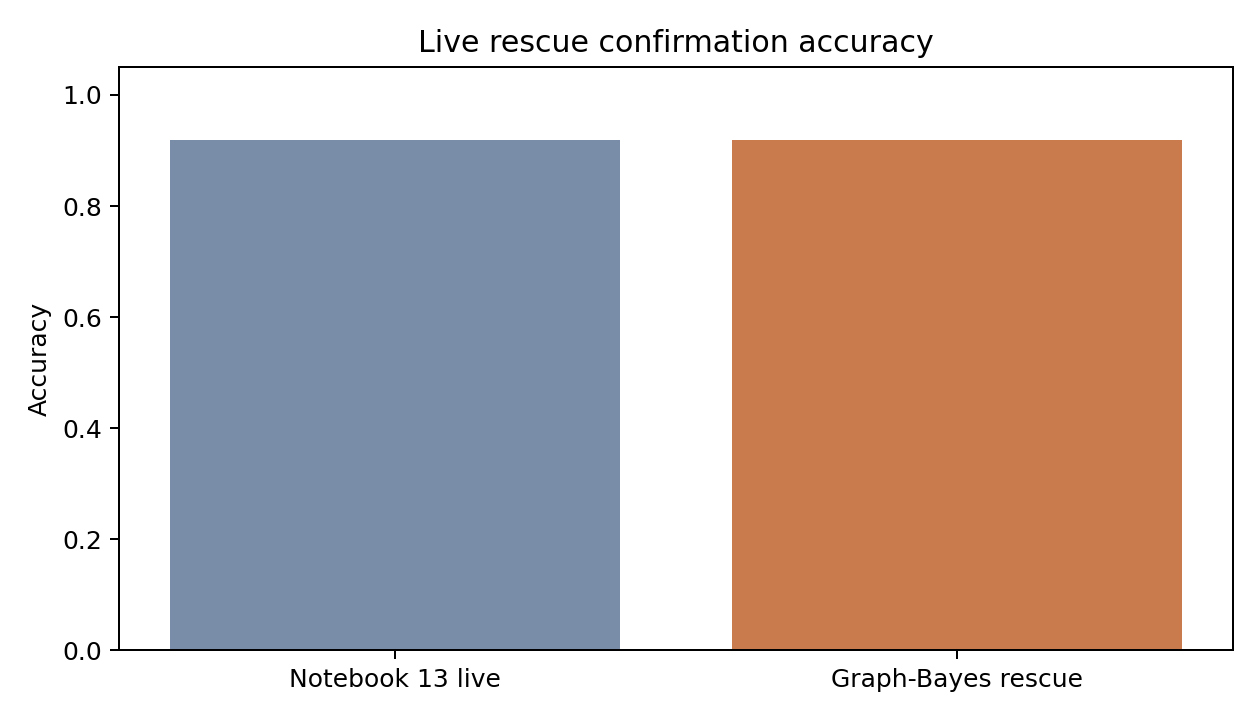
\includegraphics[width=0.70\linewidth]{artifacts/graph_algorithmic_ledger/live_graph_bayes_rescue_confirmation_49case_v1/figures/accuracy_comparison.png}
\caption{Notebook 24: live graph/Bayes rescue did not improve over the fresh base.}
\end{figure}

The honest claim is:

\begin{quote}
Graph and Bayes are useful as critics and candidate generators, but not yet a confirmed replacement for the Notebook 13 backbone.
\end{quote}

\section*{12. Notebooks 25--26: Why Branching Became Interesting}

Notebook 25 collected three more Notebook 13-style live base replicates.

Notebook 26 analyzed five trajectories total:

\begin{itemize}[leftmargin=*]
    \item Notebook 13 frozen: 43/49,
    \item Notebook 24 base: 45/49,
    \item Notebook 25 r01: 44/49,
    \item Notebook 25 r02: 42/49,
    \item Notebook 25 r03: 42/49.
\end{itemize}

Majority vote over the five trajectories stayed at 43/49. But oracle best-of-five reached 47/49.

That is the key branching insight:

\begin{quote}
The value is not broad voting. The value is selective branching at fragile states plus a good resolver.
\end{quote}

\begin{figure}[H]
\centering
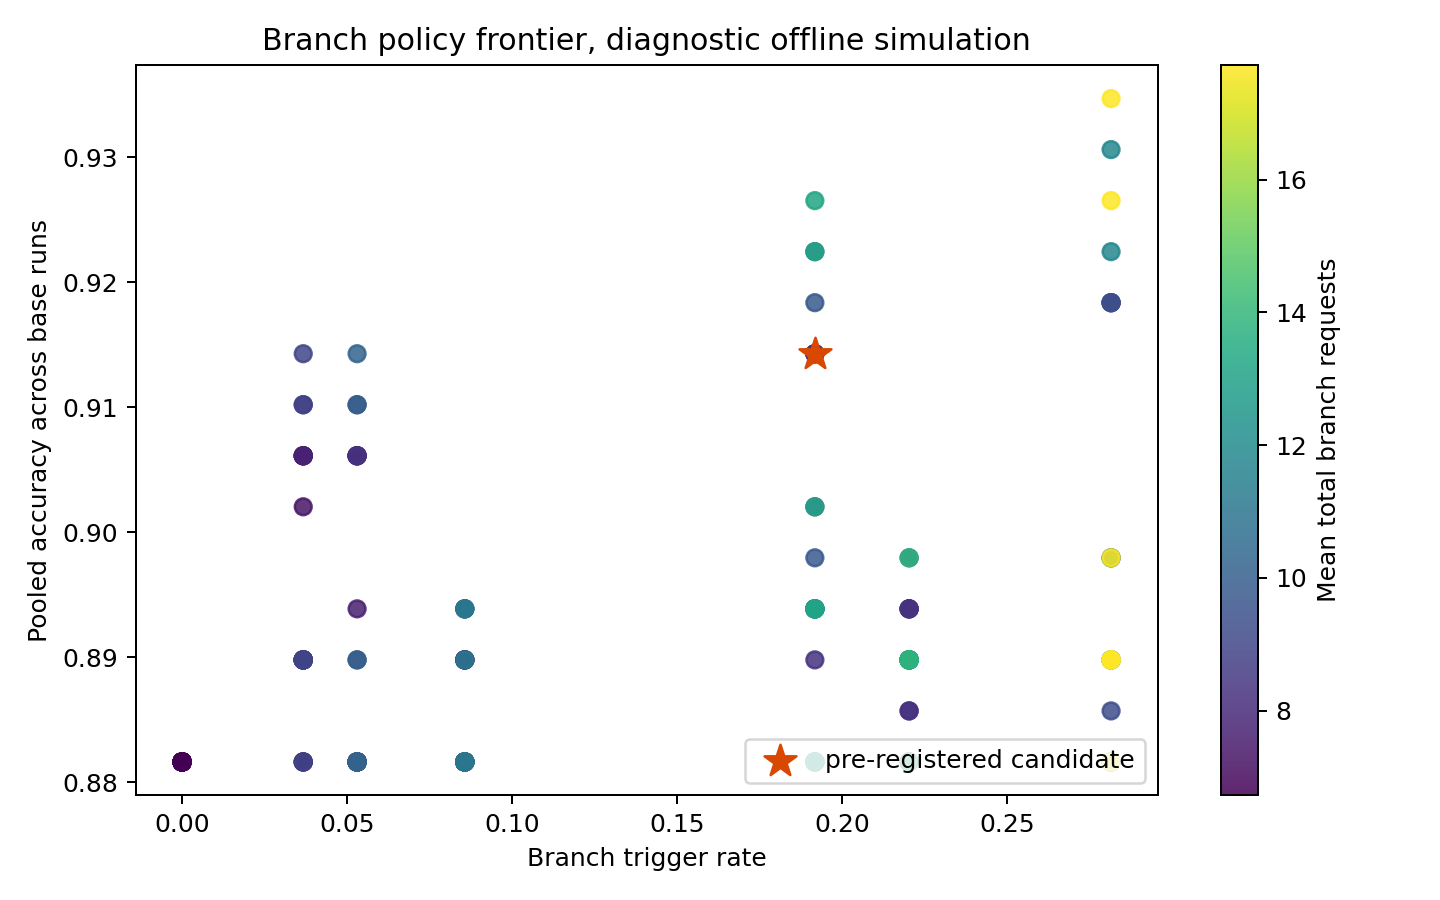
\includegraphics[width=0.76\linewidth]{artifacts/trajectory_replicates/offline_branching_trajectory_lab_49case_v1/figures/branch_policy_frontier.png}
\caption{Notebook 26: selective branch policies can recover some wrong trajectories in offline replay.}
\end{figure}

\section*{13. Notebook 27: First Live Targeted Branching}

Notebook 27 was the first prospective live branching test.

It used:

\begin{itemize}[leftmargin=*]
    \item a hand-written suspicious-state trigger,
    \item up to two fresh-context LLM branches,
    \item a raw Bayesian posterior judge.
\end{itemize}

Result:

\begin{itemize}[leftmargin=*]
    \item base branch: 42/49,
    \item targeted branching: 43/49,
    \item wins: 2,
    \item regressions: 1,
    \item mean total branch requests: 11.45.
\end{itemize}

This partially confirmed branching because it recovered Myocarditis and Panic attack. But it regressed COPD, so it was not promoted.

The failure taught us what Notebook 28 needed:

\begin{itemize}[leftmargin=*]
    \item learned branch gate instead of hand rules,
    \item graph/Bayes/MLP pseudo-candidates,
    \item base protection when the base answer is strongly graph/Bayes supported,
    \item confounder coverage for silent wrong-answer cases.
\end{itemize}

\section*{14. Notebook 28: MLP-Gated Confounder Graph/Bayes Branching}

Notebook 28 is the learned branching version.

It uses a branch-trigger MLP trained on train/validate synthetic partial states. The input features include:

\begin{itemize}[leftmargin=*]
    \item MLP confidence, margin, and entropy,
    \item graph ranks and support,
    \item Bayesian posterior and ranks,
    \item graph/Bayes/MLP agreement,
    \item request count and visible-root count,
    \item confounder-pair coverage.
\end{itemize}

The branch trigger estimates whether the base answer is likely a wrong anchor.

Validation:

\begin{itemize}[leftmargin=*]
    \item branch-trigger MLP AUC: 0.954,
    \item average precision: 0.931,
    \item selected threshold: 0.375,
    \item precision at threshold: 0.823,
    \item recall at threshold: 0.940.
\end{itemize}

The resolver also changes. It scores:

\begin{itemize}[leftmargin=*]
    \item base prediction,
    \item real branch predictions,
    \item graph pseudo-candidate,
    \item Bayes pseudo-candidate,
    \item MLP pseudo-candidate.
\end{itemize}

It also protects the base answer when the base is graph rank 1 and Bayes rank 1.

Live 49-case result:

\begin{table}[H]
\centering
\begin{tabular}{lr}
\toprule
Metric & Value \\
\midrule
Same-run base & 42/49 = 0.857 \\
Notebook 28 selected & 44/49 = 0.898 \\
Top-3 / Top-5 & 0.959 / 0.959 \\
Wins vs base & 2 \\
Regressions vs base & 0 \\
Branch trigger rate & 0.082 \\
Mean selected requests & 6.63 \\
Mean total branch requests & 9.96 \\
\bottomrule
\end{tabular}
\end{table}

This is a safer branching result than Notebook 27. It improves its same-run base by two cases and has zero regressions.

But it still is not promoted. It reaches 44/49, not the 47/49 target, and it does not beat the strongest fresh Notebook 13-style base run of 45/49.

\begin{figure}[H]
\centering
\begin{subfigure}{0.48\linewidth}
\centering
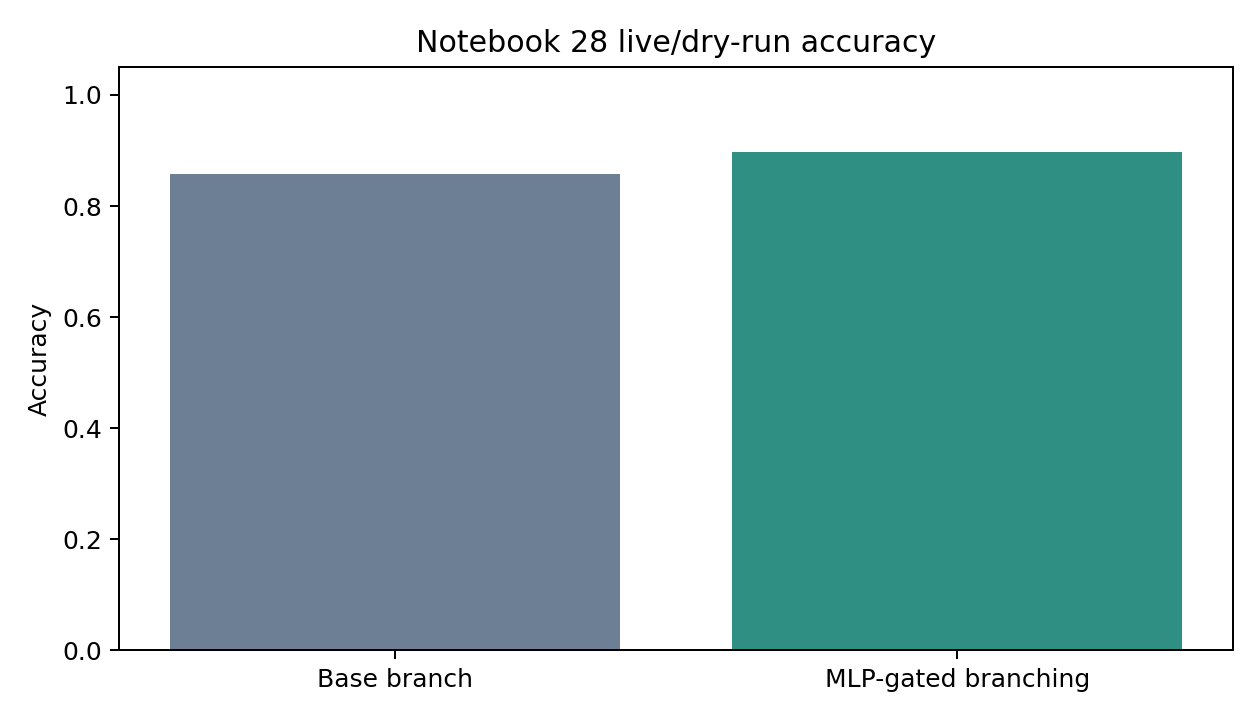
\includegraphics[width=\linewidth]{artifacts/trajectory_replicates/mlp_gated_confounder_graph_bayes_branching_49case_v1/figures/accuracy_comparison.png}
\caption{Notebook 28 accuracy.}
\end{subfigure}
\hfill
\begin{subfigure}{0.48\linewidth}
\centering
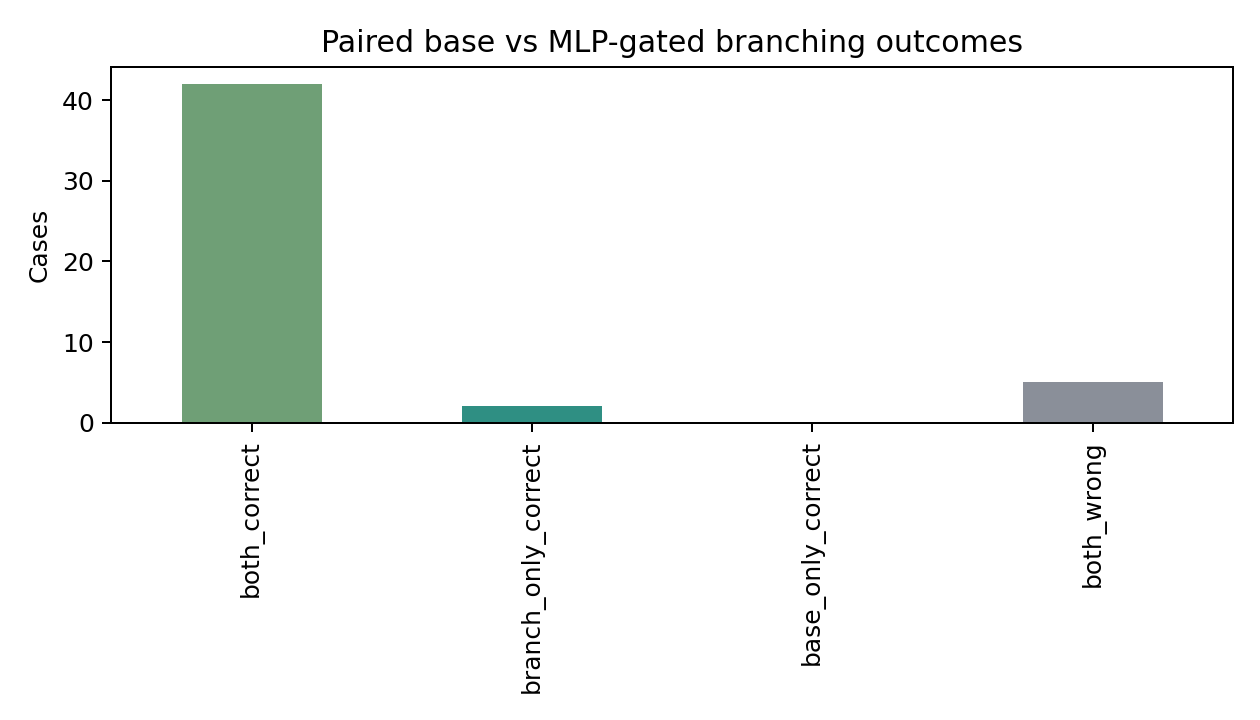
\includegraphics[width=\linewidth]{artifacts/trajectory_replicates/mlp_gated_confounder_graph_bayes_branching_49case_v1/figures/paired_outcomes.png}
\caption{Paired outcomes.}
\end{subfigure}
\caption{Notebook 28 improved over its same-run base with zero regressions.}
\end{figure}

\section*{15. Final Results Summary}

\begin{table}[H]
\centering
\resizebox{\textwidth}{!}{%
\begin{tabular}{lcccc}
\toprule
System & Cases & Accuracy & Top-5 & Request cost \\
\midrule
Initial-evidence MLP & full test & 0.378 & 0.730 & 0 \\
Full-evidence MLP & full test & 0.996 & 1.000 & all fields \\
Notebook 13 selected-stop hybrid & 49 & 0.878 & 0.939 & 6.59 \\
Notebook 24 fresh base & 49 & 0.918 & 0.939 & 6.20 \\
Notebook 23 offline rescue & 49 & 0.959 & -- & 6.96 \\
Notebook 27 live branching & 49 & 0.878 & 0.939 & 11.45 total branch requests \\
Notebook 28 learned branching & 49 & 0.898 & 0.959 & 9.96 total branch requests \\
\bottomrule
\end{tabular}
}
\end{table}

The final defended method remains the Notebook 13-style backbone: LLM evidence acquisition under a deterministic ledger, with MLP-guided stopping.

Notebook 28 is important, though. It shows a safer version of branching: learned gate, pseudo-candidates, and base protection. But it is still not strong enough to replace the backbone.

\section*{16. Likely Technical Questions}

\textbf{What is the partial-evidence MLP used for?}

It is used as a belief monitor. It gives confidence, margin, entropy, top-k predictions, and agreement signals from the current partial evidence state. In Notebook 13, it is mainly used for stopping.

\textbf{Why not use only the MLP?}

The MLP is good at scoring visible evidence, but it is not automatically good at deciding what to ask next. Notebook 14 showed direct MLP question selection did not promote.

\textbf{Why not use only the LLM?}

The LLM is good at choosing questions, but LLM-only stopping used more evidence or became brittle. The MLP gives a more stable stop signal.

\textbf{Why did Bayesian VOI fail?}

It selected globally informative but generic fields and created trajectories that differed from the partial-evidence MLP training distribution. So the posterior idea was sound, but this controller was not.

\textbf{What did graph methods add?}

They added support and contradiction signals. Graphs were not good as a hard question controller, but they were useful as final critics, rescue features, and branch resolver features.

\textbf{What did branching prove?}

Branching proved that some wrong trajectories can be recovered by alternate workups. But it did not prove multi-agent superiority. Notebook 28 made branching safer than Notebook 27, but it still did not beat the strongest base run.

\section*{17. Final Closing}

My final defended statement would be:

\begin{quote}
We built a reproducible DDXPlus baseline ladder and a controlled sequential diagnostic workup system. The defended backbone uses an LLM to acquire evidence under a deterministic ledger, and a partial-evidence MLP to decide when enough evidence has been gathered. It performs far above the initial-evidence baseline while asking only about 6 to 7 evidence fields. The graph, Bayesian, and branching notebooks show promising algorithmic directions, especially Notebook 28's learned branch gate, but the promoted method remains the evidence-efficient Notebook 13-style LLM-plus-MLP workup.
\end{quote}

\end{document}
